% !TEX root=../main.tex

\section{Editors: interaction with the end user}

We claim to create a language to model \emph{interactive} workflows.
We define interaction as
\begin{quote}
  communication with the end user of the system.
\end{quote}
The way to communicate with the user in our language is an \emph{editor}.
Using an editor,
a user can enter information into the system,
clear it, reenter it et cetera.
Editors may or may not contain a current value.
When an editor has a value, it can be \emph{changed} or it can be \emph{cleared}.
When it is empty, a value can be \emph{filled}.
This is depicted as a state diagram in \autoref{fig:editor-state} below.

\begin{figure}
  \centering
  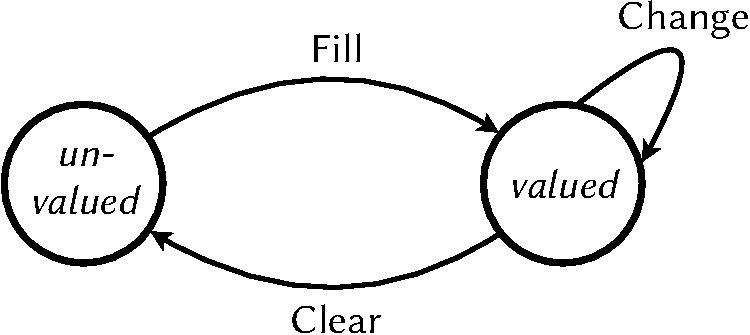
\includegraphics[width=0.5\textwidth]{figures/editor-state-crop.pdf}
  \caption{State of an editor and its possible transitions}
  \label{fig:editor-state}
\end{figure}

For this purpose, we extend our task language with two constructs:
a valued editor $\Edit e$ and an unvalued editor $\Fill \beta$.
%, which contains the expression $e$, which expects a value of type $\tau$.
\begin{grammar}
  Pretasks
    & p & ::=& \ldots      & \\
    &   &\mid& \Edit e     & – valued editor \\
    &   &\mid& \Fill \tau  & – unvalued editor \\
\end{grammar}
Some examples:
\begin{itemize}
  \item $\Edit 2$ is a valued editor with value $2$.
  \item $\Fill \String$ is an unvalued editor.
    The user can enter something of type $\String$.
  \item $\Edit ((\lambda x . x)\ 5)$ is a valued editor which,
    after evaluation, will contain the value $5$.
\end{itemize}

Valued editors contain an expression $e$.
Therefore they inherit the type of $e$,
but embedded in the container type $\Task$.
For now, we only accept expressions of a basic type $\beta$ as a value of an editor.
This is expressed by the following typing rule for a valued editor.
\begin{equation*}
  \userule{T-Edit}
\end{equation*}

Empty editors do not have a value,
but, because we strive to a fully typed system,
we like to assign a type to them.
We have two options to solve this:
\begin{enumerate*}
  \item let the empty editor have a polymorphic type;
  \item annotate empty editors with a type and use that.
\end{enumerate*}
The first option sounds appealing, however, consider the following use case.
We start with an editor containing the value two: $\Edit 2$.
The user can change this value, as long as it is an integer,
for example to five: $\Edit 5$.
Clearing the value results in an empty editor: $\Fill$.
Now, is the user allowed to enter a value of some other type?
That is, can we now enter a string?
This would change the type of the editor!
We need to keep track of the type of values that can be entered into an empty editor
and therefore we choose to annotate them with a type.
The typing rule becomes:
\begin{equation*}
  \userule{T-Fill}
\end{equation*}


\subsection{Events}

To interact with an editor,
we should interact with the user with some kind of interface.
In a graphical setting,
we can present the user an input box.
The user can than change and clear values continuously.
In a text oriented world,
we can print out the current value of an editor
and prompt the user for a new value
or a command to clear the editor.

To abstract away from the user interface,
we introduce an event system.
It does not matter how these events are sent to the application.
This can be by pushing a button,
entering text in an input box,
committing some text on a command line,
or sending it over a web socket.

We define a new syntactic category of \emph{events} $\eta$.
For now, they only contain \emph{actions} $\alpha$,
we will introduce new events in a later section.
As we already discussed before,
there are two actions that can be handled by editors:
\begin{enumerate*}
  \item changing the value; or
  \item clearing the value.
\end{enumerate*}
\begin{grammar}
  Events
    & \eta   & ::=& \alpha & – action \\
  Actions
    & \alpha & ::=& v      & – change editor to value \\
    &        &\mid& \Empty & – empty an editor \\
\end{grammar}
The value of an editor, empty or not, can be changed to a value $v$ by just sending the value as an event.
To clear a valued editor, we send the $\Empty$ action.

Handling events is done by a new semantic relation.
This relation takes a task $t$ and an event $\eta$ which results in a new task $t'$.
We write
\begin{equation*}
  \boxed{\RelationH}
\end{equation*}
Formalising our intuition from previous paragraphs,
we need three rules to describe the transitions of editors.
\begin{equation*}
  \userule{H-Change} \qquad \userule{H-Clear} \qquad \userule{H-Enter}
\end{equation*}
Note that the conditions to the right of the rules take care of typing.
They make sure the type of the entered value and the type of the editor are the same.


\subsection{Example}

Now, we can make a still dull but interactive example of a workflow.
How could an interactive session with the user look like when we start with a simple workflow with one editor,
containing the value two?\todo{We should probably add a rule that doesn't change a task when the event doesn't match\ldots}
\begin{align*}
    & \Edit 2 \\
  \handle{5} & \hint{change value to five} \\
    & \Edit 5 \\
  \handle{\Empty} & \hint{clear the current value} \\
    & \Fill \Int \\
  \handle{50} & \hint{enter the value fifty} \\
    & \Edit 50 \\
  \handle{\astring{Bye}} & \hint{changing the value to a string won't work\ldots} \\
    & \Edit 50 \\
  \handle{10} & \hint{change value to ten} \\
    & \Edit 10
\end{align*}
